\chapter{Preliminaries: Background}
\label{chapter:background}

This chapter presents the concept of static analysis, shortly summarises the JavaScript language and its static analysis approaches, and gives insights to the background technologies of the previously mentioned \emph{Codemodel-Rifle} framework.


\section{Static Analysis}

\subsection{Introduction}

Static source code analysis is a software testing approach performed without compiling and executing the program itself. Usually the source code of the analysed software first gets transformed to a mathematical data structure — which is mostly a tree or a different form of graph —, then the data structure is inspected by automated tools with the goal of finding software defects. As static analysis is performed without actually executing the program, software can be analysed in as early as its source code state, before getting to testing or deployment.

Techniques for static analysis exist for almost 50 years~\cite{emanuelsson2008comparative}. A 1995 research paper concludes, that \textquote{Static analysis is effective and complementary to dynamic testing. Hence its use is to be recommended in the context of the majority of critical software.}~\cite{373902} In 2017, open- and closed-source static analysis tooling is quite extensive, and publicly available not only for the academia and the commercial industry, but for open-source projects as well~\cite{wikipedia-static-analysis}.

The sophistication and the generated reports' quality of static analysis tools vary: some report potential fault locations, others use mathematical tools to verify properties of a software and its specification. Besides general code quality-related applications, static analysis acquires a growing market share also in safety- and mission-critical systems for exploring defects~\cite{livshits2006improving}.


\subsection{Source Code Transformation}

Software source code is a text, usually consisting of human-readable characters. Characters formulate sequences of instructions by the specified grammar of the programming language. To be executed on a computer, most programming languages need to be \emph{compiled} by a \emph{compiler} first, meaning the source code has to be transformed into a \emph{binary code} or \emph{bytecode} to be executed. Other languages, called interpreted languages, do not need to be compiled, they are interpreted and executed at runtime.\footnote{JavaScript is an interpreted language.}

Compiled languages' are always analysed, at least at compilation time by the compiler. If the software contains severe errors (like type association errors in strongly typed languages), the compiler will abort its operation, thus the software can not be run, since it has not been compiled. Considering interpreted languages do not need to be compiled, they are not analysed by a compiler before running, and — generally — not analysed at all. Interpreted languages' static analysis is therefore beneficial to compensate the lack of a compiler-like component in the software processing chain.

More than one static analysis methods can be run simultaneously on a project. As static analysis inspects the source code without modifying the original, the operations of several such tools are independent from each other. Therefore at compiled languages, added static analyses can only compliment the compiler's necessary analysis.

Usually three abstract data structures are used to represent software source code in a mathematically defined form.


\subsubsection{Abstract Syntax Tree (AST)}

If the compiler or an analysis tool processes the source code and its parser transforms the source code into an abstract data structure, it usually creates an \emph{Abstract Syntax Tree}. It is the tree-representation of the code, meaning every node in the tree is a semantic element of the source code. The \emph{source code to AST transformation} is vica versa unambiguous, meaning the two structures are identical to each other regarding the program logic. It is abstract in the sense of syntax: not all elements of the syntax is preserved in its AST, meaning without the language grammar, transformation would not be possible.


\subsubsection{Abstract Semantic Graph (ASG)}

A more abstract representation of the source code (or an AST) can be an \emph{Abstract Semantic Graph}. Derived semantic information added to the AST can result in a graph which provides more insights into the structure of the program: it can reveal data about variable and function scopes, and much more to be detailed later.


\subsubsection{Control-Flow Graph (CFG)}

Control-Flow Graphs or Execution Graphs contain execution path of a program. They are essential to compiler optimisations and widely used in static analysis tools.


\subsection{Use Cases and Limitations}

Static analysis use cases are generally code quality-related: on the one hand, the program under development should comply to specified programming styles and rules, on the other hand, the number of defects in the software should be as low as possible, ideally zero. If the software under development is part of a mission-critical solution, finding and fixing defects is essential.

Code style analysers and code formatters are used to enforce team- or company-wide coding styles. Linters are rule-based tools and are used to reveal simple programming errors and poorly used programming constructs. Pattern-matching techniques supplemented with algorithms to manipulate the representing data structure can be efficient to obtain deeper insights of the source code: this approach is to be detailed later being one of the subjects of this thesis. Static analysis with methods of formal verification uses mathematical models and methods to prove well-defined statements about the inspected source code.

Static analysis is limited in many ways. It often provides false values: \emph{false positives} are issues which do not have real significance or are not even true, \emph{false negatives} are real issues not being reported by the analysis tool. A framework is considered to be \emph{sound} if all defects checked for are reported by the tool: there are no false negatives but there can be false positives. A general approach of static analysis frameworks is to be sound, and simultaneously avoid extensive reporting of false positives~\cite{emanuelsson2008comparative}.

Regarding limitations, time and resources are also important aspects. An analysis tool can not be utilised efficiently, if the amount of either time or resources consumed by an analysis is too high. Even if it was theoretically possible to create a tool which finds every possible defects in a piece of source code, this tool would presumably consume so much time and resources for an analysis that there would be no appropriate use case for operating it~\cite{anderson2008use}.

Exploring execution paths greatly benefits static analysis proceedings, as it provides extra information about program states. Nevertheless, exploring all possible execution paths of a program is very costly: if a procedure contains $n$ branches without loops, the number of intraprocedural execution paths would be $2^n$~\cite{anderson2008use}. And even if a tool would encapsulate so much resources that it would be capable of exploring all possible executions paths, the set of possible inputs, whose cardinality is typically infinite, of the software would still not be taken into account. Since Alan Turing proved the halting problem to be generally undecidable over Turing-machines, we can conclude that, generally, some questions about a software can not be answered only by inspecting its source code.


\section{JavaScript}

JavaScript is a high-level, run-time interpreted language, featuring object-oriented capabilities. Being part of the core of the World Wide Web~\cite{flanagan2006javascript}, it is the most commonly used programming language in the world in 2016~\cite{javascriptstackoverflow}.


\subsection{Brief History of JavaScript}

Like all new technologies, JavaScript evolved very fast in the beginnings. The basics of the language was developed in 10 days by Brendan Eich, then-employee of Netscape Communications~\cite{10.1109/MC.2012.57}. The language had multiple names over the time: first it was Mocha, then LiveScript, then in December 1995, it was renamed to JavaScript as a sort-of marketing movement~\cite{webedjavascripthistory}, after seeing the then-popularity of Sun Microsystems' heavyweight Java language.

Initially, non-professional programmers were aimed by the idea to provide a portable, embeddable programming language that can be interpreted in web browsers. Since the syntax was closely similar to the syntax of C / C++ / Java, JavaScript rapidly gained traction: in the time of writing this thesis, it is the most used programming language in the world~\cite{javascriptstackoverflow}. It features browser-based client- and separate runtime-based server-side capabilities~\cite{nodejs} as well, and extensive tooling, package management~\cite{npmjs}, testing and build systems are available for automated operations in even larger software development organisations.


\subsection{The \es as a Standard and as a Language}

There is a significant aspiration to standardise the JavaScript language with its core capabilities and data structures. The first intentions of standardisation began in 1997 by Ecma International~\cite{webedjavascripthistory}, resuling in \emph{Standard ECMA-262}~\cite{ecmascriptstandardfirstversion}. The newest standard currently is the \emph{ECMA-262, 7\textsuperscript{th} Edition (ES7)}~\cite{ecmascriptstandard}. Apart from standardisation, there are several implementations of JavaScript in interpreters, like Chakra\footnote{\texttt{https://github.com/Microsoft/ChakraCore}}, JScript\footnote{\texttt{https://msdn.microsoft.com/library/hbxc2t98.aspx}} and Google's V8\footnote{\texttt{https://github.com/v8/v8}}~\cite{stein-daniel-msc}.

Today's growing traction of standardised JavaScript, henceforth also referenced as \es, can be explained with several reasons. Due to being untyped\footnote{In JavaScript, no static types are assigned to entities.} and dynamic\footnote{Meaning of dynamic here: contrary to static languages where compilation time checks play an important role in verifying various properties of the program, dynamic languages' several common programming behaviours are executed only at run-time. Considering a common example: in JavaScript we have the \lstinline{eval()} function to execute source code at run-time.}, static analysis of JavaScript is difficult. The \es standard enhances plain JavaScript with several new programming structures making the language more expressive and sometimes more simple~\cite{es6-features}. Users of the language can write more coherent code by applying these new language constructs as well as best practices making it easier to interpret the program by a static analysis tool.


\subsection{The Process of Transpiling}

\emph{Transpiling} is a word came into existence by mixing \emph{transforming} and \emph{compiling}. It is a generally used process in the \es developer community to ensure backwards compatibility of newer \es language standards, like ES6 and ES7.

\paragraph{Compiler}

A \emph{compiler} is a software with the primary goal of transforming software source code written in a high-level programming language into machine language, usually into a form of binary code called object code~\cite{pcmagcompilers}. Compiled languages, like C, C++, Java, or C\#, need to be compiled to be executed on a specific processor architecture.

\paragraph{Transpiler}

A \emph{source-to-source compiler} or \emph{transpiler} is a software which transforms software source code written in a high-level programming language into another high-level programming language. Ideally the two source codes are logically equivalent, meaning that with given abstractions, the operation of the two different software is the same.\footnote{The two executed programs need to be logically equivalent, but do not need to correspond in every technical aspects: there can be differences in machine-level operations and low-level proceedings.}

Transpiling and compiling have a set of common processing steps~\cite{kulkarnitranspiler}. First the source code is parsed into an abstract mathematical format for effective manipulation, then, after optimisations and transformations, both methods yield another kind of code. While compilers' output, being low-level machine code, can be generally executed on a computer architecture without further transformation steps, transpilers' output need further processing. Considering transpiling interpreted languages', the main use case is to provide compatibility with older or other versions of the language.

\begin{table}[!htbp]
	\newcommand{\fullsupport}{\tikz\draw[black,fill=black] (0,0) circle (0.8ex);\xspace}
	\newcommand{\partialsupport}{\tikz\draw[black,fill=none] (0,0) circle (0.8ex);\xspace}
	\newcommand{\nosupport}{—}
	\centering
	\begin{tabular}{l|cccc}
		\toprule
		                                    	&     \textbf{Chrome 58}     &     \textbf{IE 11}     &     \textbf{iOS 9}     &     \textbf{Android 5.1}     \\
		\midrule
		\textbf{default function parameters}  &     \fullsupport           &      \nosupport        &     \nosupport         &     \nosupport               \\
		\textbf{spread (…) operator}          &     \fullsupport           &      \nosupport        &     \partialsupport    &     \nosupport               \\
		\textbf{for..of loops}                &     \fullsupport           &      \nosupport        &     \partialsupport    &     \partialsupport          \\
		\textbf{const}                        &     \fullsupport           &      \partialsupport   &     \partialsupport    &     \partialsupport          \\
		\textbf{let}                          &     \fullsupport           &      \partialsupport   &     \nosupport         &     \nosupport               \\
		\textbf{arrow functions}              &     \fullsupport           &      \nosupport        &     \nosupport         &     \nosupport               \\
		\bottomrule
	\end{tabular}

	\caption{Excerpt from an \es 6 compatibility table~\cite{kangax}}
	\label{table:ecmascript-compatibility}
\end{table}

In the JavaScript scene, compatibility is a ubiquitous problem, see \Cref{table:ecmascript-compatibility}. Considering all the different browsers and server runtimes, and the slow progression of adopting JavaScript standards, transpiling has an important role in ensuring that the software works on a broad scale of platforms: code written in a modern syntax like ES6 can easily be transpiled into an universally supported syntax like plain JavaScript.

\Cref{fig:transpiling-example} shows two logically equivalent pieces of code: the second one (plain JavaScript) is created by transpiling the first one (\es 6) with a popular, automated transpilation tool, \emph{babel}\footnote{\texttt{http://babeljs.io}}. As the example shows, new language constructs can make the code much more concise, while the transpiled alternative provide compatibility with older desktop browsers and server runtimes.

\vspace{1em}
\begin{figure}[!htb]
	\centering
	\begin{minipage}{25em}
		The first piece of code uses ES6 constructs for simplicity:

		\begin{lstlisting}[language=JavaScript]
		[1, 2, 3].map(n => n ** 2);
		\end{lstlisting}

		The second piece of code uses widely-supported plain JavaScript constructs only, and is created by transpiling the first piece of code with \emph{babel}:

		\begin{lstlisting}[language=JavaScript]
		[1, 2, 3].map(function (n) {
		  return Math.pow(n, 2);
		});
		\end{lstlisting}
	\end{minipage}
  \caption{A transpilation example}
  \label{fig:transpiling-example}
\end{figure}


\subsection{Looking into the Goals of JavaScript Static Analysis}

As JavaScript is an interpreted language not being checked by a compiler by default at compilation time~\cite{373902}, it is recommended to apply static analysis during the development of, or before deploying a JavaScript application. Due to its dynamic and untyped\footnote{TypeScript, a strict superset of JavaScript adds static typing to the language~\cite{typescript-website}.} nature~\cite{flanagan2006javascript}, static analysis for the language is a challenging task. There are several existing approaches focusing mainly on defects detection~\cite{madsen2013practical, livshits2010gulfstream, jensen2009type}, but few of them are ready for production usage, and most of them lack compatibility with recent \es versions.

Being untyped, an obvious analysis goal is type inference: checking type correctness can eliminate several defects from software. Security demands imply that deeper, logical analysis of JavaScript code is needed. Besides security, the development procedure itself can also benefit from static analysis: there are features like automatic stub generation or auto-complete~\cite{madsen2013practical} in several development tools~\cite{esprima-autocomplete, webstorm-autocomplete}.


\section{Graph Databases}

Being graphs, developing new data structures for Abstract Syntax Trees, Abstract Semantic Graphs and Control-Flow Graphs would be superfluous: they can be practically stored in graph databases. There are established vendors on the open-source and also on the closed-source market~\cite{ibm-graph, arangodb-graph, datastax-graph, neo4j-website, orientdb-graph} providing databases with either a native graph storage model, or with support for storing graphs over an underlying data model other than a graph. For manipulating data, they provide well-defined and well-documented interfaces instead of ad-hoc solutions.

Graphs are mathematically well-defined data structures being broadly used in several fields of computer science. Recent technologies and implementations made possible for developers to easily embed graph data models into their applications. There are numerous real-world scenarios which can be represented more efficiently as graphs (\emph{nodes} connected to each other via \emph{edges}), than with the traditional, relational approach.

\subsection{The Property Graph Data Model}

It is a common way to define graphs as a set of objects, in which some object pairs are connected to each other. In this model, an object is called \emph{vertex} or \emph{node} or \emph{point}, and a connection between two \emph{vertices} is called \emph{edge} or \emph{relation}. Connections can be detailed further by specifying their directionality, also they can be \emph{labeled} to define them even more. Similarly labeling vertices leads to the model of \emph{typed graphs}. If we assign properties to the nodes or relations, we get the model of \emph{property graphs}. Properties, as shown in \Cref{fig:property-graph}, are usually key-value pairs in the format of \lstinline{key = `value'}. Generally, keys are strings, and values represent common data types like string, integer, float, etc.

\begin{figure}[!htb]
	\centering
	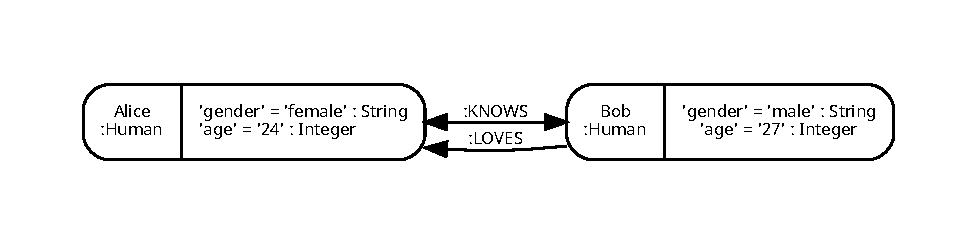
\includegraphics[width=\textwidth, trim=1cm 1cm 1cm 1cm,clip]{figures/property-graph.pdf}
	\caption{Two people's relationship modeled with a property graph}
	\label{fig:property-graph}
\end{figure}

The Codemodel-Rifle framework uses property graphs for its internal data storage. The parsed source code's AST is transformed into an ASG, and is stored as a property graph: nodes in the AST become property graph nodes, nested AST nodes are connected to each other via labeled graph relations. \Cref{fig:codemodel-rifle-asg} shows the ASG of the following JavaScript program: \lstinline{const PI = 3.141593;} produced and visualised by Codemodel-Rifle.\footnote{Administrative properties and labels are omitted for the sake of simplicity, e.g. no identifiers are shown.}

\begin{figure}[!p]
	\centering
	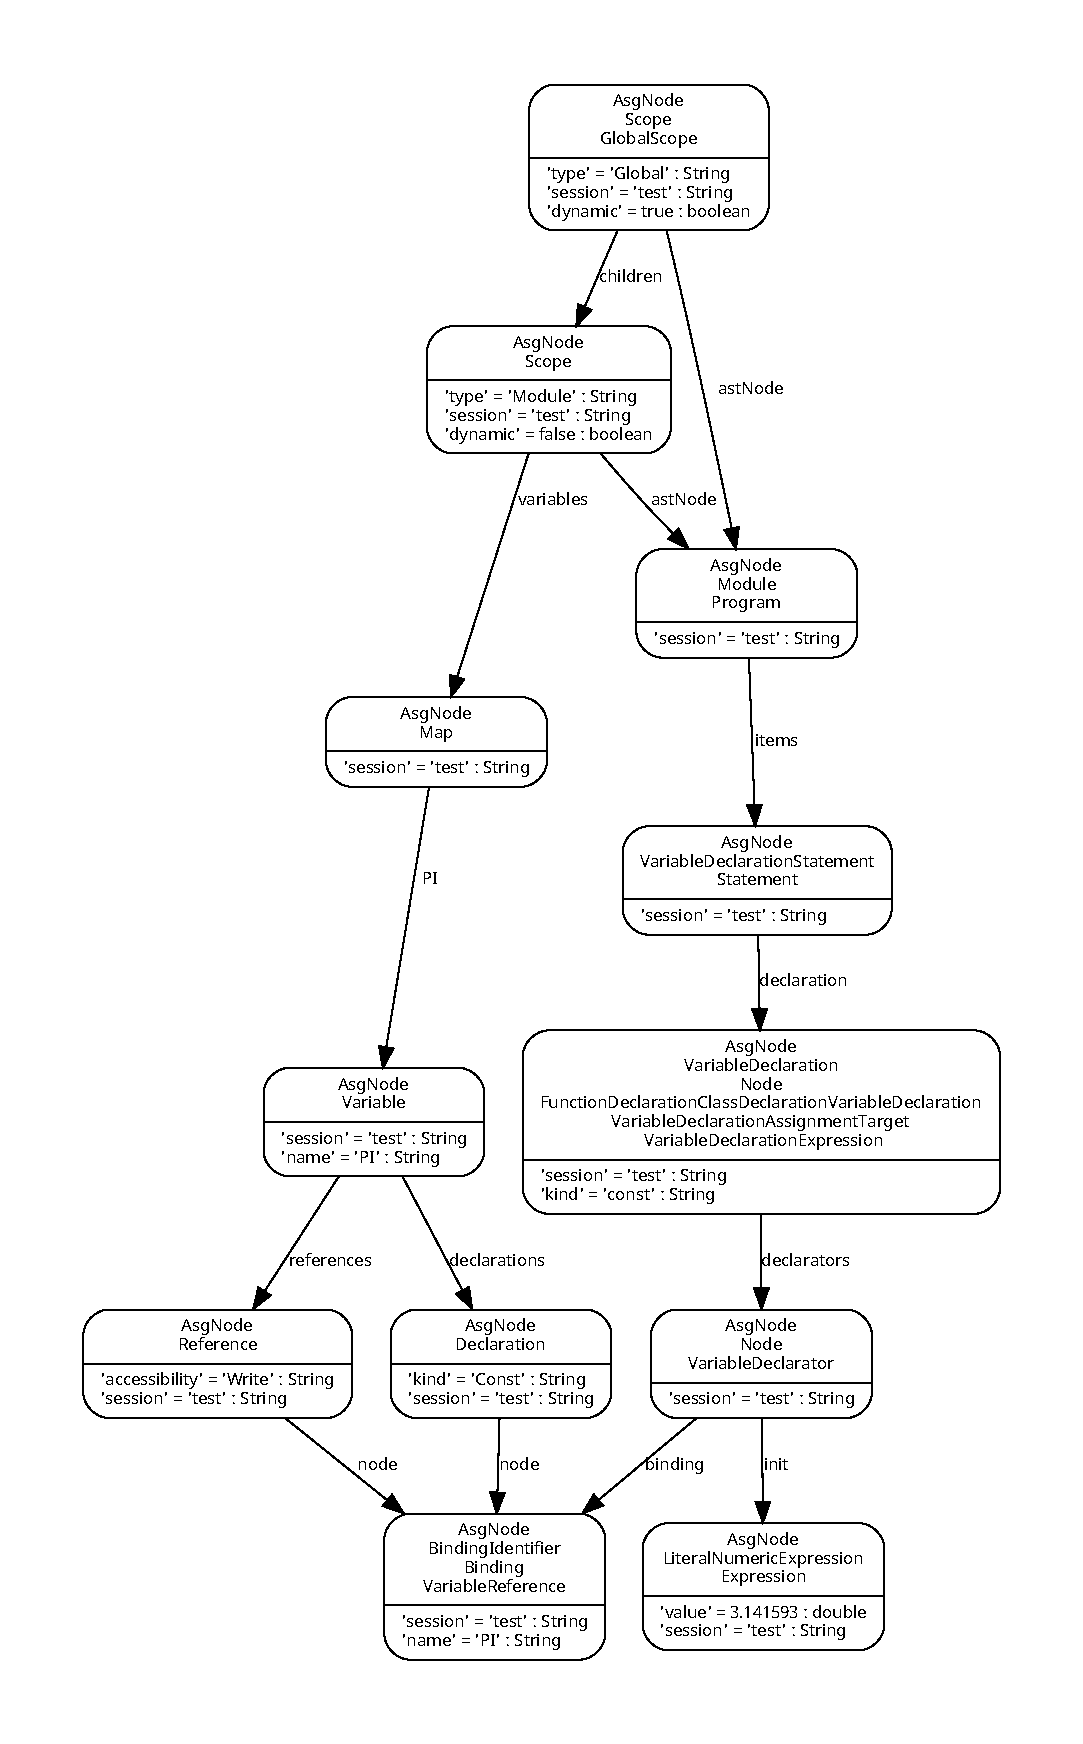
\includegraphics[height=\textheight, trim=1cm 1cm 1cm 1cm,clip]{figures/codemodel-rifle-asg.pdf}
	\caption{\lstinline{const PI = 3.141593;} in Abstract Semantic Graph format}
	\label{fig:codemodel-rifle-asg}
\end{figure}

\subsection{Neo4j}

Amongst a handful of graph database vendors~\cite{graph-dbs}, Neo Technology's Neo4j is the most popular one~\cite{graph-dbs-raking}. It features a pure graph data model, contrary to other vendors' multi-model approaches. Besides Neo Technology, Neo4j is backed by the open-source community as well~\cite{neo4j-github}. There are two variants: \emph{Community Edition} and \emph{Enterprise Edition} with an extended feature set. Interestingly, open-source licensing is available for the Enterprise Edition as well~\cite{neo4j-opensource}, for closed-source software, commercial licensing is available~\cite{neo4j-licensing}.

Neo4j provides two access models, detailed in the following paragraphs.

\paragraph{Embedded mode} For JVM-based languages, a native API is exposed for data operations with a very low latency. This makes the database directly embeddable to any software written in a JVM-compatible language, but provides less scalability than the \emph{server mode}.

\paragraph{Server/Remote mode} The database can be operated as a separate server listening on its binary \emph{Bolt} protocol as well as on its HTTP REST interface. From scalability aspects, the Enterprise Edition's master-slave database replication\footnote{At the time of this writing, multi-master replication is not offered by Neo4j~\cite{neo4j-clustering-architecture}.} is only available in server mode.

The Codemodel-Rifle framework uses Neo4j for its property graph storage. At first, the database was embedded into the software, but due to licensing issues, the framework had to be refactored to use Neo4j in server mode.\footnote{The licensing issues and the details and results of the refactoring are described in Section 3.1.}

\subsection{Cypher}

Cypher is a query language developed especially for graph databases by Neo Technology~\cite{neo4j-cypher}. Contrary to the usage of the native API, it is mostly used when Neo4j is deployed in server mode. \Cref{fig:cypher-intro} shows that the language uses a sort of ASCII-art to represent nodes and relationships: nodes are in parentheses, relationships are in brackets surrounded by relationship direction information.

\begin{figure}[!htb]
	\centering
	\lstinline{(Bob)-[:LOVES]->(Alice)}
  \caption{A basic Cypher example}
	\label{fig:cypher-intro}
\end{figure}

Cypher syntax is elegant and expressive, thus very readable. Besides using it to represent nodes and relationships, we can utilise it to access the database's indexing capabilities and stored procedures. Since complex pattern-matching conditions can be expressed easily and intuitively in Cypher, it should be the primary way of accessing Neo4j instead of the little bit faster but less readable API.\footnote{Since the subject of this thesis mainly features Cypher queries, Cypher is detailed further in Chapter 5.}


\section{Running Example}

In this section I provide a set of \es codes as a software defect example, which accompanies the reader throughout the thesis. This example is to be used whenever a new static analysis concept is introduced. There are two files in the example: \lstinline{exporter.js} and \lstinline{importer.js}.

The first one exports a function, which happens to return $0$, as a variable. The second one imports the variable and tries to divide a number with the return value of the imported function variable. Through this example, I present that this and similar software defect cases can be revealed by static analysis, even if the defect spans more than one \es modules (source files), and includes patterns which can not be matched by one generalised pattern description. \Cref{fig:running-example-exporter} presents \lstinline{exporter.js}. \Cref{fig:running-example-importer} presents \lstinline{importer.js}.

\begin{figure}[!htb]
	\begin{lstlisting}[language=JavaScript]
					var a = 0;

					export default function b() {
					  let c = function d() {
					    return a;
					  };

					  return c();
					};
	\end{lstlisting}
  \caption{\lstinline{exporter.js} module}
  \label{fig:running-example-exporter}
\end{figure}

\begin{figure}[!htb]
	\begin{lstlisting}[language=JavaScript]
					import defaultName from "exporter";

					let a = 5 / defaultName();
	\end{lstlisting}
  \caption{\lstinline{importer.js} module}
  \label{fig:running-example-importer}
\end{figure}

%%% Local Variables:
%%% mode: latex
%%% TeX-master: "../main"
%%% End:
